%!TEX root = Thesis.tex
\chapter{State of the Art}
The following chapter covers an overview and analysis of existent solutions in the related research areas of web-based third-party applications, which were designed specially for retrieving different type of sensed data. At the beginning of the chapter in the Section 3.1 the most familiar research works are studied. It covers public and private sector, that mainly focused on data retrieving through the Web.

In the section 3.2 the prominent approaches of frontends development are studied and evaluated against the requirements described in the section 2.1 with a purpose to clarify their capabilities and properties.  

All solutions discovered in the this chapter are evaluated against the requirements described in the section 2.1.

\section{Web of Sensors}
 This thesis is targeted at the creation of a generic user-friendly interaction system. Nowadays every project is focused on a specific area of realization and handling a narrow range of data types, such as urban environment\cite{song2010real} or real-time environmental monitoring portal or geospatial infrastructure to efficiently collect and serve a vast field of a data over the web\cite{6588063} and much more as described above. A lot of work related to Cloud-based information resources and Internet of Things(IoT), where the main focus on information which is the result of human behaviour or usage of already implemented tools ot platforms.  

	\emph{Smart city}\cite{6588063} tool using information technology and communication (ICT) to help local government to monitoring what currently happened in the city(Figure 3.1). Web-based application for monitoring city in single dashboard to help summarize the current condition of a city. The architecture system use network sensor consisting of sensor nodes that has function to capture city condition like temperature, air pollution, water pollution, traffic situation. Also exist a possibility to add another information e.g., socio-economic situation like public health service, economic indicator, energy supplies, etc. The results of work presents a prototype of the smart city dashboard the give more accurate information of Bandung City, one of big cities in Indonesia. It consists of network sensor, server, application and also communication protocol which is used for city monitoring. The summary information of city can be displayed in single view to help people watching, analyzing and action to what being happen at the real-time in the city.
	  \begin{figure}[!ht]
		\centering
		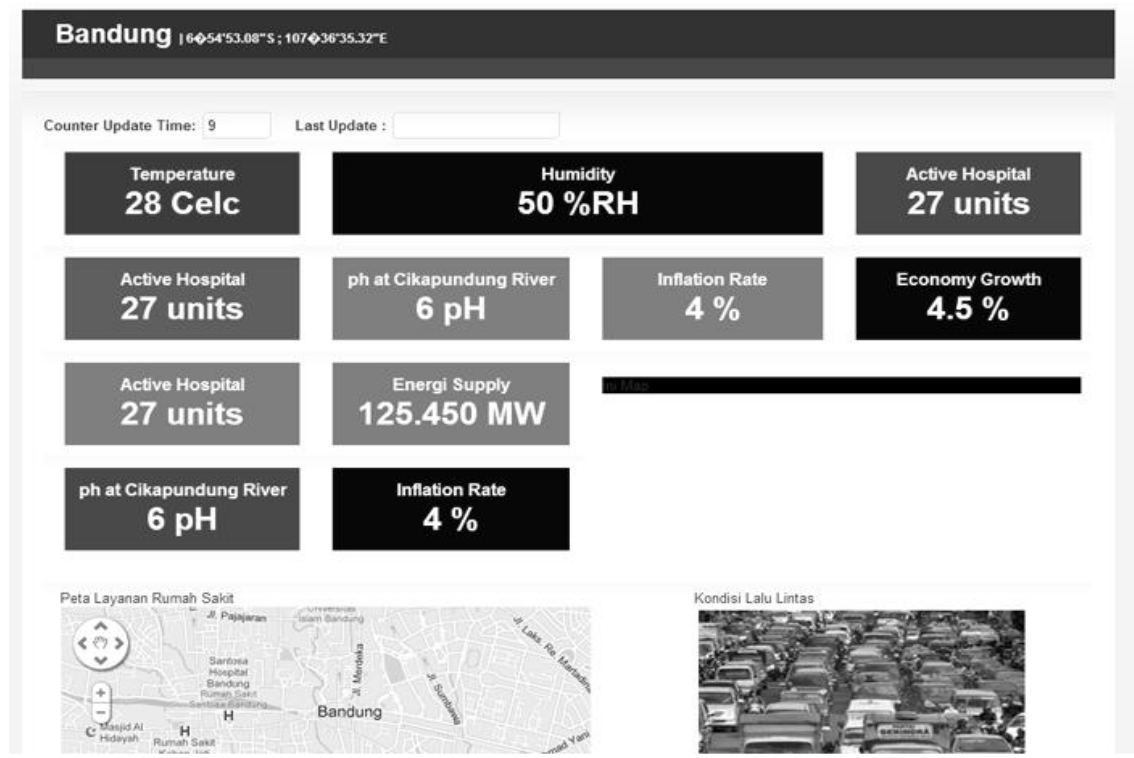
\includegraphics[scale=0.4]{Material/examples/SmartCity.png}   
		\caption[Sample of Smart City Dashboard Application]{Sample of Smart City Dashboard Application}                  
		\end{figure}

	\emph{Microsoft SensorMap\cite{10.1109/MC.2007.250}}has proposed a system to monitor, search and visualize spatially and geographically related data such as driving directions, directory entries, weather and traffic conditions based on Microsoft Virtual Earth and overlay with housing prices, crime rates, bus locations, and other data on top of browsable maps. SensorMap is a Web portal that allows owners of sensor networks to register their physical sensors and publish their data on SensorMap. They use GeoDB to store the sensor network information, housing sensor metadata including the publisher's name; the sensor's location, name, and type; the data type; and freetext descriptions. DataHub to retrieve the new sensor data to enable real time services. The aggregator to summarize sensor data in a specific area to clients. And SensorMap GUI is based on Windows Live Local and therefore provides features such as zooming, panning, street maps, satellite images, and 3D views. In addition, it lets end users pose queries on available sensors. SensorMap currently supports three types of queries: geographic queries that drawing geometric shapes directly on the map specifies (for example, within a region, near a route); type queries that sensor types specify within the viewport; and freetext queries that keywords describing sensors specify.

	 \emph{LiveWeb Portal}\cite{yang2011liveweb} presents the architecture, design, and approach to build a sensorweb service portal, where sensorweb is a global observation system for varied sensor phenomena from the physical world and the cyber world measured in a real-time. This system has been used to represent and monitor real-time physical sensor data and cyber activities from ubiquitous sources. LiveWeb meets its goal of providing an efficient and robust sensor information oriented on a web service, enabled with real-time data representation, monitoring and notification. LiveWeb has the following properties: the system enables sensorweb service accessible from anywhere, makes sensor network data readable by anyone, provides methodology of building searching engine and sensor network sharing. Based on open standards in the world of web, they propose an approach of how to build a generic system with heterogenious resources.

	\emph{Internet of Things}\cite{bendel2013service} presents a service platform based on the Extensible Messaging and Presence Protocol (XMPP) for the development and provision of services for Internet of Things(IoT) mainly focusing on the integration of things based on service technologies, scenarios in domains like smart cities, automotive or crisis management require service platforms involving real world objects, backend-systems and mobile devices. And argued necessary usage of XMPP client as protocol for unified, real-time communication and introduce the major concepts of a platform. Based on two case studies demonstrated real-time capabilities of XMPP for remote robot control and service development in the e-mobility domain. And in the same time a proof of concept was made by authors in a project called ACDSense\footnote{ACDSense project, \url{http://www.rwth-aachen.de/}} that XMPP and its numerous extensions have gained momentum as a multi-purpose lightweight middleware for social computing, multi-device interaction, and communication with sensors(Figure 3.2). The concept was demonstrated with a use case of three distributed and interconnected XMPP-driven pervasive systems: standard XMPP client, sensor App, Web browser sensors dashboard. The aggregation of data as a Web application done by using multiple widgets with the help of an Inter-Widget Communication(IWC) approach based on portlets\cite{ACDSense}.
	    \begin{figure}[!ht]
		\centering
		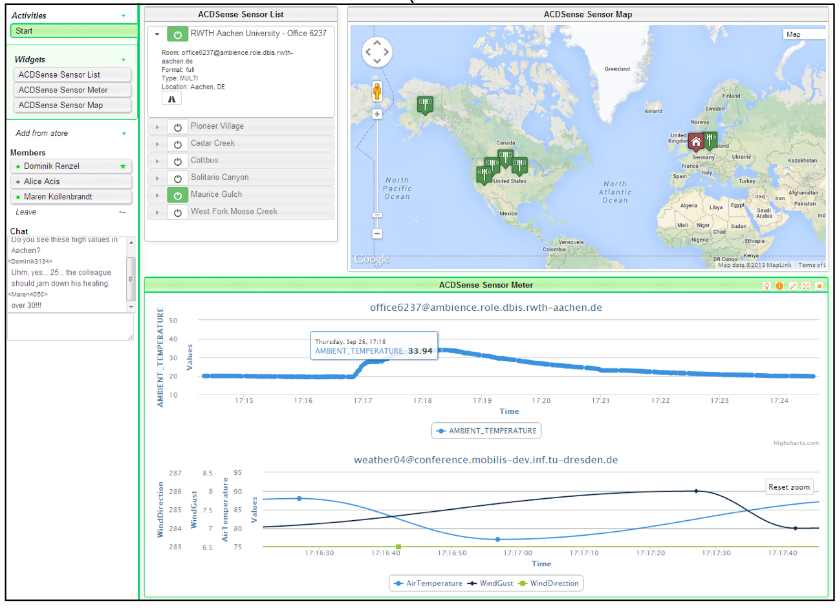
\includegraphics[scale=0.6]{Material/examples/ACDSense.png}   
		\caption[Sample of ACDSense]{Sample of ACDSense}                  
		\end{figure} 

	\emph{Dynvoker Portal}\cite{spillner2008ad} a generic human-driven ad-hoc usage approach, by including rapid service testing and dynamic inclusion of services as plugins into applications. Dynvoker is an engine, which consists of a relatively small application core which can be run as a servlet, a web service or a command-line application. Explore method-centric and resource-centric services alike, output forms in various formats or integrate GUI services to provide a richer user experience. The generic design of many parts of Dynvoker has yielded a lightweight architecture which is freely available to any interested person as an open source project.

	\emph{Sensor Web Enablement} project\cite{ogc} is focused on developing standards to enable the discovery of sensors and corresponding observations, exchange, and processing of sensor observations, as well as the tasking of sensors and sensor systems. Open Geospatial Consortium(OGC), Inc. members specifies interoperability interfaces and metadata encodings that enable real-time integration of heterogeneous sensor web into the information infrastructure. Developers will use these specifications in creating applications, platforms, and products involving Web-connected devices such as flood gauges, air pollution monitors, stress gauges on bridges, mobile heart monitors, Webcams, and robots as well as space and airborne earth imaging devices. In this publication by OGC was defined such an important XML-based standards as: Sensor Model Language (Sensor ML), Sensor Observation Service (SOS), Web Notification Service (WNS) etc. As subproject calls SANY(Sensors Anywhere) focuses on interoperability of in-situ sensors and sensor networks. The goal for the SANY architecture is to provide a quick and cost-efficient way to reuse data and services from currently incompatible sensors and data sources in future environmental risk management applications. By developing a standard open architecture and a set of basic services for all kinds of sensors, sensor networks, and other sensor-like services, the SANY IP supports and enhances both GMES (Global Monitoring for Environment and Security, a major European space initiative) and GEOSS (Global Earth Observation System of Systems) in the area of in situ sensor integration. Though the SANY work enhances interoperability for monitoring sensor networks in general, the application focus is on air quality, bathing water quality, and urban tunnel excavation monitoring.
 
    \emph{VICCI Project}(Visual and Interactive Cyber-physical Systems Control and Integration)\cite{vicci,6548811}(Figure 3.3). The scope includes smart home environments and supporting people in the ambient assisted living, considers the software-technical side of so-called "Cyber-physical systems" (CPS). This term includes complex, embedded systems, which connect the virtual and the physical world with each other(IoT) in different application scenarios. The main uses of CPS are in logistics, traffic optimization, in the use of robots in the industrial and domestic sectors, in modern energy networks (Smart grid), in the building and factory automation (Smart factory), as well as in the field of intelligent office installations (Smart Office). The aim of project VICCI is the creation of software engineering principles that are necessary for the development of complex cyber-physical systems. Firstly, CPS should be made understandable and accessible by means of a comprehensive control center. Secondly, platforms that enable the development and marketing of software for complex CPS through a pure control panel are to be developed. A domestic environment is considered a sample scenario in which a person with reduced mobility is supported by sensors, actuators and a service robot, which is currently seen as a complex cyber-physical system. No concrete frontend or any kind of user-friendly GUI have been not yet developed.
     \begin{figure}[!ht]
		\centering
		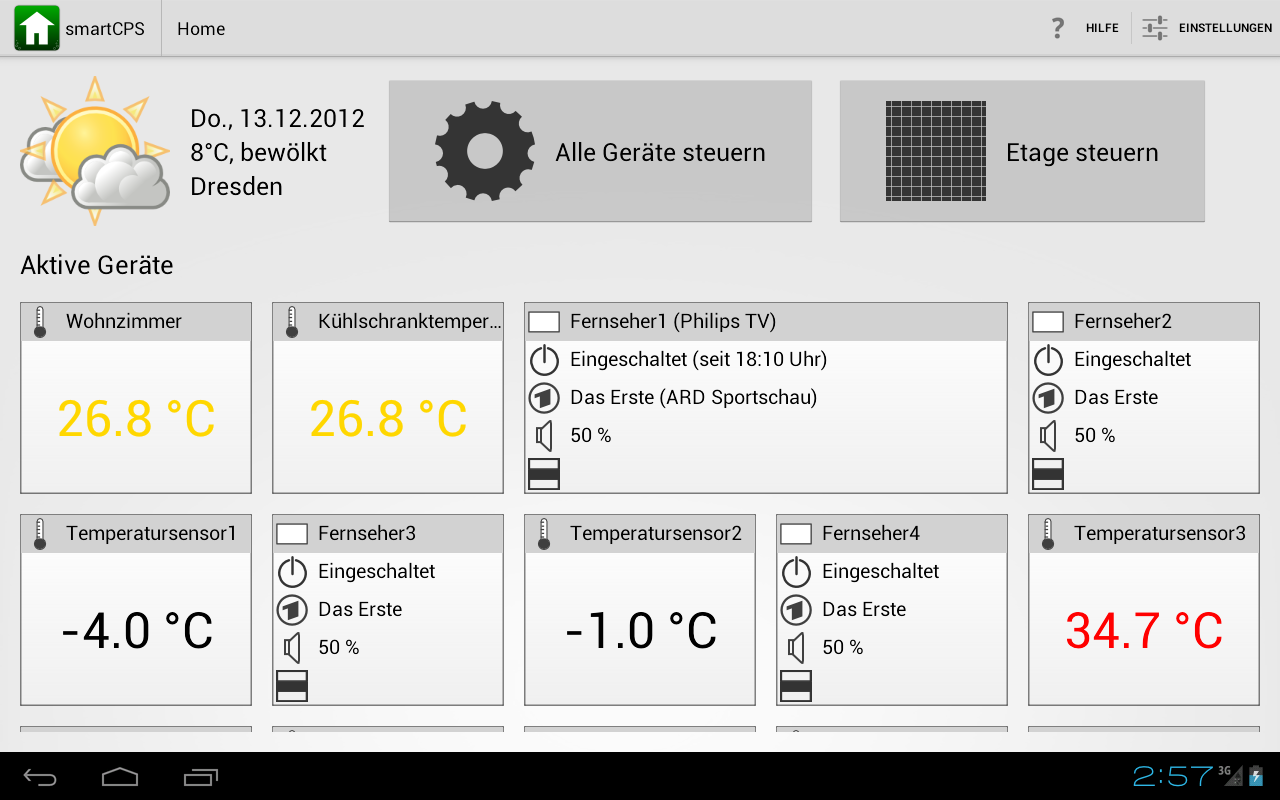
\includegraphics[scale=0.4]{Material/examples/VICCI.png}   
		\caption[Mockup of VICCI project]{Mockup of VICCI project}                  
		\end{figure} 

	A series of articles devoted to integrate sensed data into a Cloud. Special attention is given to privacy-relevant or otherwise sensitive information that is stored in a Cloud. 

	\emph{SensorCloud}\cite{hummen2012cloud}, a cloud design for user-controlled storage and processing of sensor data proposed security architecture enforces end-to-end data access control by the data owner reaching from the sensor network to the Cloud storage and processing subsystems as well as strict isolation up to the service-level. In this paper authors presents transport security mechanisms for communication with the Cloud, applies object security mechanisms to outbound data items, and performs key management for authorized services. 

	\emph{CloudRemix\cite{spillner2013personal}} a Personal and Federated Cloud Management Cockpit, an interactive cockpit to manage personal clouds and their federations(Figure 3.4). Is a new techniques for users to perform asset discovery, exchange and management in Cloud area. The CloudRemix prototype demonstrates its utility to manage personal clouds in both social and market-driven environments. The goal of CloudRemix is to be open, user-centric regarding the manageable assets, and flexible regarding their free or commercial exchange, with or without explicit contract negotiation. CloudRemix is an open-source web-based cockpit application with support for multiple users. Each user gets to see an aggregated list of both local and remote services of each of the asset types.
	    \begin{figure}[!ht]
		\centering
		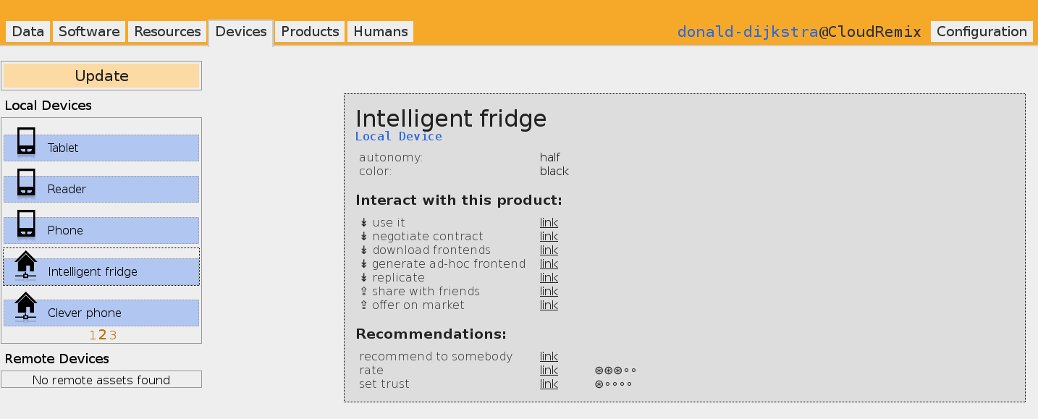
\includegraphics[scale=0.6]{Material/examples/CloudRemix.png}   
		\caption[Sample of CloudRemix]{Sample of CloudRemix}                  
		\end{figure} 

    \emph{SensorMap}\cite{nath2006challenges} is a portal web site for real-time real world sensor data(Figure 3.5). 
		SensorMap allows data owners to easily make their data available on the map. The platform also transparently provides mechanisms to archive and index data, to process queries, to aggregate and present results on a geo-centric web interface based on Windows Live Local. In this position paper  described the architecture of SensorMap, key challenges in building such a portal, and current status and experience. Is an ongoing project with the goal of creating an online searchable portal of live data from the physical world.
		\begin{figure}[!ht]
		\centering
		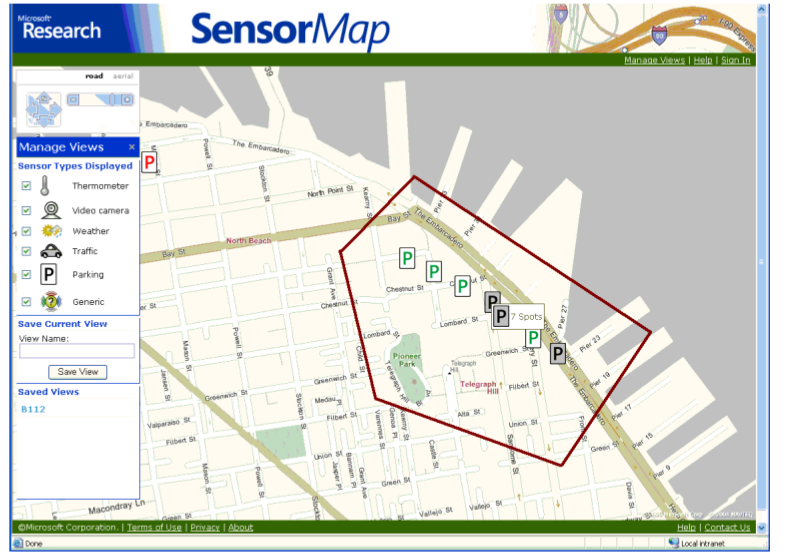
\includegraphics[scale=0.5]{Material/examples/SensorMap.png}   
		\caption[Sample of SensorMap]{Sample of SensorMap}                  
		\end{figure}
		 Example services provided by such a portal include: a Parking Space Finder service, for directing drivers to available parking spots near their destination; a Bus Alert service, for notifying a user when to head to the bus stop; Waiting Time Monitors, for reporting on the queuing delays at post offices, food courts, etc.; a Lost and Found service, for tracking down lost objects; and a Person Finder service, for locating colleagues or monitoring children playing in the neighborhood. The GUI is based on Windows Live Local, and therefore shares its attractive features such as zooming, panning, street maps, satellite images, etc. In addition, it lets end-users to pose queries on available sensors. SensorMap currently supports three types of queries: geographic queries specified by drawing geometric shapes (e.g., a region, a route) directly on the map, type queries specified by sensor types within the viewport, and free text queries specified by keywords describing sensors. It overlays the results returned from the agregator on Windows Live Local. The SensorMap lets users query data sources and view results on the map. The SensorMap describes first constructive idea how to interconnect different types of sensors available in the Web through API and provides system architecture. But within this project authors don't consider questions as: retrieval of real sensors in a room, sensor control, live data streaming, adaptive GUI and integration with another platform and systems without specifically added libraries. 
  
    \emph{Xively Cloud Services}\footnote{Xively ,\url{https://xively.com/}} is the Public Cloud which was particularly built for Internet of Things, by giving developers standards-based services and tools, elastic scalability, and intuitive lifecycle management capabilities oriented on a business customer. With Xively, user can gain the agility and efficiency needed to rapidly meet market demands for compelling connected products and solutions. Xively's Platform as a Service (PaaS) provides the tools and services needed to create compelling products and solutions on the Internet of Things.
    \begin{figure}[!ht]
		\centering
		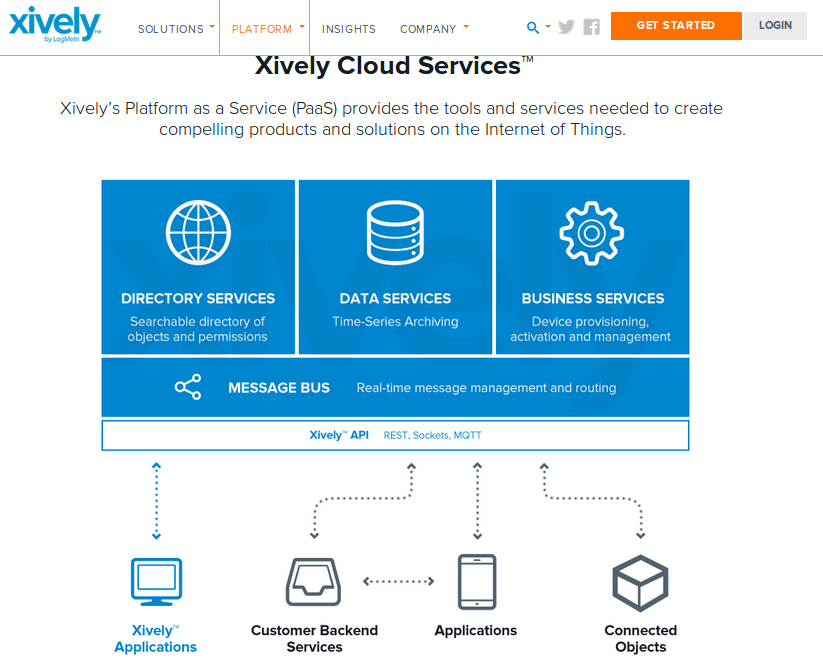
\includegraphics[scale=0.5]{Material/examples/Xively.png}   
		\caption[Sample page of Xively]{Sample page of Xively}                  
		\end{figure} 

    \emph{Optique}\footnote{Optique ,\url{http://www.optique-project.eu/}} is a scalable semantic access to Big Data for effective data analysis and value creation. Optique brings about a paradigm shifted for data access: by providing a semantic end-to-end connection between users and data sources; enabling users to rapidly formulate intuitive queries using familiar vocabularies and conceptualizations; seamlessly integrating data spread across multiple distributed data sources, including streaming sources; exploiting massive parallelism for scalability far beyond traditional RDBMSs and thus reducing the turnaround time for information requests to minutes rather than days\cite{calvanese-etal-JAIR-2013-explanation,ernestojimenezruizbernardocuencagrau2013ontology,DBLP:conf/dlog/MollerNOW13ohneCross}. According to research publications, no research was done in a field of visualization and presentation. Implemented Frontend with adaptive and cross-browser GUI was developed specifically for this project by using up-to-date technologies (jQuery, HTML and CSS).
    \begin{figure}[!ht]
		\centering
		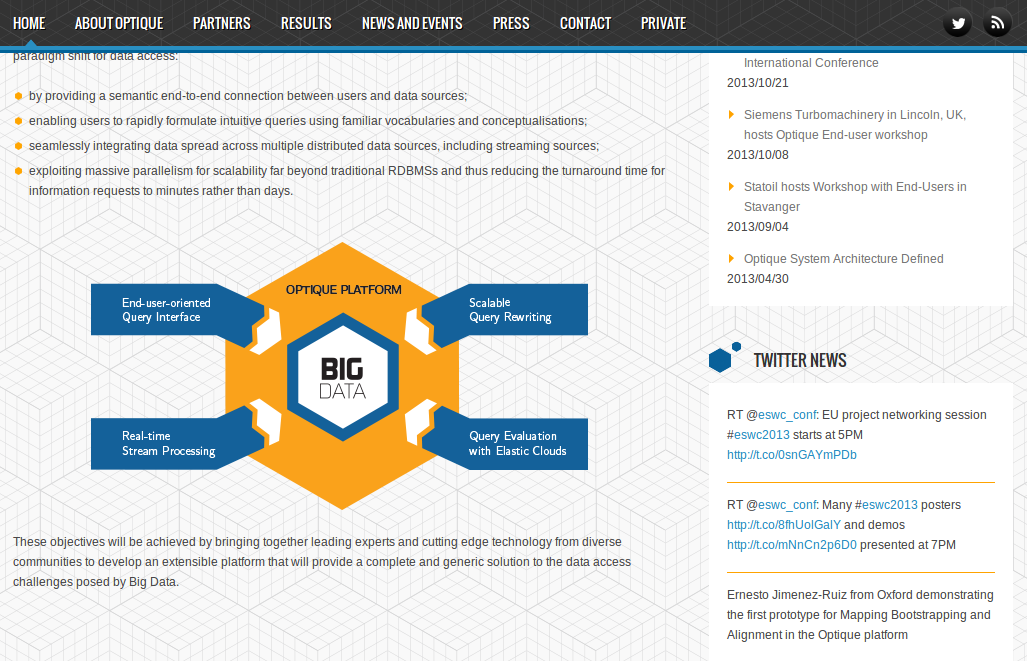
\includegraphics[scale=0.5]{Material/examples/Optique.png}   
		\caption[Sample page of Optique]{Sample page of Optique}                  
		\end{figure} 

    All research projects are presented in Table 3.1 according to such characters as: status(active or inactive in nowadays), availability of Frontend as full functional system with logic and GUI, Mockup(planed GUI), type of project(public or private).

    \begin{table}[H]
	\centering
	\begin{tabular}{|r|l|l|l|l|l|}
	\hline
	Target 			       & Status & Frontend & Mockup & Type of Project \\
	\hline 
	\hline
	Smart City		       & active & yes & yes & public \\
	\hline
	Microsoft Sensor Map   & inactive & yes & - & private \\
	\hline
	LiveWeb Portal	       & inactive & no & no & public \\
	\hline
	Sensor Web Enablement  & inactive & no & no & public \\
	\hline
	SensorCloud		       & inactive & no & no & public \\
	\hline
	CloudRemix		       & active & yes & - & public \\
	\hline
	VICCI Project		   & active & no & yes & public \\
	\hline
	Dynvoker Portal		   & inactive & no & no & public \\
	\hline
	Internet of Things	   & active & no & no & public \\
	\hline
	SensorMap              & inactive & no & no & public \\
	\hline
	Xively                 & active & yes & - & private \\
	\hline
	Optique                & active & yes & - & private \\
	\hline
	ACDSense               & active & yes & yes & public \\
	\hline
	\end{tabular}
	\caption[State of the Art]{State of the Art Summary}
	\label{tab:state_of_the_art}
	\end{table}

Among all researched projects presented not interactive frontends was implemented only to satisfy concreate requirements from a backend. Most of them simply visualise data provided by backend, no manipulation can be done in such a way. Only few of them have interactive web-based interfase, such as ACDSense or CloudRemix, but unfortunately, due to concreate realization, no enhancement on frontend side(adding new modules, new visual parts) can't be done independently from technology used on a backend side. Most of the research projects have no frontend at all, or only some mockup as .jpg picture. Thus, concluding all researched projects above, become clear that the needs of a generic frontend, that can be easily integrated with any type of data-driven platform is high. To do so, needed to be clarify what are the main methodologies to build frontend are existent nowadays, specify types of data that have to be retrieved and possible interface for aggregation of data and collaboration between all modules defined by system architecture.

\section{Frontend Development Approaches}
In computer science, the frontend is responsible for collecting input from user and processing it to a backend system and another direction - collecting data from backend, namely sensor data steam, and processing it to the user-friendly interface. Therefore, on the one side, generic frontend has to satisfy architecture requirements from backend, such as: fine-grained structure, cross-platforming, loose coupling; and on the other side, implement a dynamic user-friendly interface to a end-user with a client-side multi-user data binding. Thus, to satisfy aforementioned requirements it is necessary to compare all available web-oriented solutions.

To retrieve data from different resources in one web-based interface was specified next existent approaches :
\begin{itemize}
 \item portal with portlets,
 \item mashup\footnote{\url{http://www.programmableweb.com/applications}},
 \item browser based systems,
 \item non-browser based system
\end{itemize}

	\subsection{Portal}
		The main concept is to present the user with a single web page that brings together or aggregates content from a number of other systems or servers. 

		Usually, each information source gets its dedicated area on the page for displaying information (a portlet); often, the user can configure which ones to display. The extent to which content is displayed in a "uniform way" may depend on the intended user and the intended purpose, as well as the diversity of the content. Very often design emphasis is on a certain "metaphor" for configuring and customizing the presentation of the content and the chosen implementation framework and/or code libraries\cite{pautasso2008restful,seong2006usability}. In portal technologies end-user can customize number of retrieved data sources, but for that he has to be aware what is it and how to integrate it in portal. User interface in portals have fixed layout, style and location on the web page. To make changes in it, end-user needs to have a deep knowledge of the system architecture and of whole portal entirely. The portal allows the administrator to define specific sets of applications, which are presented to the user in a single page context. The Portlets themselves are more than simple views of existing Web content. A Portlet is a complete application having multiple states and view modes, plus event and messaging capabilities.

		Portlets run inside the Portlet container of a portal server, similar to a servlet running on an application server. The Portlet container provides a runtime environment in which portlets are instantiated, used, and finally destroyed. Portlets rely on the portal infrastructure to access user profile information, participate in window and action events, communicate with other portlets, access remote content, look up credentials, and store persistent data.

		A portal may use a search engine API to permit users to search intranet content as opposed to extranet content by restricting which domains may be searched. Apart from this common search engines feature, web portals may offer other services such as e-mail, news, stock quotes, information from databases and even entertainment content. Portals provide a way for enterprises and organizations to provide a consistent look and feel with access control and procedures for multiple applications and databases, which otherwise would have been different web entities at various URLs. The features available may be restricted by whether access is by an authorized and authenticated user (employee,member) or an anonymous site visitor.

		Examples of early public web portals were AOL, Excite, Netvibes, iGoogle, MSN, Naver, Indiatimes, Rediff, Sify and Yahoo!\footnote{Yahoo!,\url{http://pipes.yahoo.com/pipes/}}. See for example, the "My Yahoo!" feature of Yahoo! which may have inspired such features as the later Google "iGoogle" (soon to be discontinued). The configurable side-panels of, for example, the modern Opera browser and the option of "Speed Dial" pages by most browsers continue to reflect the earlier "portal" metaphor.

		\textbf{Main features}
		\textbf{Integration} — Ability to integrate with your current tools or the possibility of adding new tools. You have your outlook calendar and email integrated within intranet.

        \textbf{Security} — Enable user or group based security to secure documents and sites throughout the intranet portal.

		\textbf{Customization} — Software that is flexible to allow for organization. Web Parts can be used to create custom modules which can make interaction easier with the site. Ability for users to customize tools and resources they use most often.

		\textbf{Collaboration} — People are now able to collaborate their work with each other. Example would be multiple people working on one document.

		\textbf{Communication Channels} — Allows corporations to promote corporate culture and present information in a more interactive way than before.

		\textbf{User Friendly} — Application must be easy to use and understand due to a wide range of technical abilities.

		\textbf{Remote Access} — Ability for users to access content away from the office.

		\textbf{Targeted Content} — Business portal administrators can target content by business group area, e.g., HR, Marketing, Legal, Corporate Executives, etc.

		Portal technology has proven powerful but complex. Mashups offer the other extreme - simplicity, but maybe not as much power. 

	\subsection{Mashup}

		Mashup is a web page, or web application, that uses content from more than one source to create a single new service displayed in a single graphical interface. The term implies easy, fast integration, frequently using open application programming interfaces (API) and data sources to produce enriched results that were not necessarily the original reason for producing the raw source data. The term mashup originally comes from pop music, where people seamlessly combine music from one song with the vocal track from another-thereby mashing them together to create something new. The main characteristics of a mashup are combination, visualization, and aggregation. It is important to make existing data more useful, for personal and professional use. To be able to permanently access the data of other services, mashups are generally client applications or hosted online. Both commercial products and research prototypes have a broad range of features that simplify a mashups design process, and provide mashups storage and publication. But to customize retrived resources end-user have no option, as use only predefined type and numbers of applications, that was created by application or platform developer. 
		The mashup application is a composite Web 2.0 application that aggregates and integrates heterogeneous web resources offered in a form of available Web APIs and sources for creating a new service. Mashups differ from traditional component-based applications in providing more situational character of these applications\cite{yu2008understanding}. In general there distinguish the following three types of mashups\cite{ibrahim2012framework}. Customer mashups are aimed at the combination and reformation data from various public sources according to users’ needs. Data mashups aggregate similar types of resources from diverse sources into a new single data representation. And business, or enterprise, mashups define composite applications that are focused on solving heterogeneous business problems by supporting collaborative activities\cite{hoyer2008enterprise}. The architecture of a mashup is divided into three layers:
		 \newline
		 \begin{itemize}
		\item \emph{Presentation / user interaction:} this is the user interface of mashups. The technologies used are HTML/XHTML, CSS, Javascript, Asynchronous Javascript and XML (Ajax).
		\item \emph{Web Services:} the product's functionality can be accessed using API services. The technologies used are XMLHTTPRequest, XML-RPC, JSON-RPC, SOAP, REST.
		\item \emph{Data:} handling the data like sending, storing and receiving. The technologies used are XML, JSON, KML.
		\end{itemize}

		Concerning architectural styles of mashup applications, server-side and client-side mashups are distinguished. In server-side mashups a content aggregation is realized on a server\cite{mashA}. The server plays a role of a proxy between the mashup application and other web sites that involved in this application. The opposite client-side mashups aggregate content on a client, typically, at a client's web browser\cite{mashB}.

	 Server-side mashup is similar to traditional Web applications using server-side dynamic content generation technologies like Java servlets, CGI, PHP or ASP. The data from multiple sources are aggregated at the server side and the final results are rendered at the client’s browser. In the client-side mashup, content mashed can be generated directly within the client’s browser using client-side scripts (such as JavaScript or Applets). Mashups following the client-side style are often referred as Rich Internet Applications (RIAs). The benefit of client-side mashup includes the prompt response to user interactions because the data is pre-processed at the client’s browser by leveraging Ajax techniques. For example, a page can be updated for portions of its content without having to refresh the entire page. Often a mashup uses a combination of both the server-side and the client-side style to achieve the data aggregation\cite{bolin2005end}.

        \textbf{Portal vs Mashup}

		Mashups and portals are both content aggregation technologies. Portals are an older technology designed as an extension to traditional dynamic Web applications, in which the process of converting data content into marked-up Web pages is split into two phases: generation of markup "fragments" and aggregation of the fragments into pages. Each markup fragment is generated by a "portlet", and the portal combines them into a single Web page. Portlets may be hosted locally on the portal server or remotely on a separate server.

		Portal technology is about server-side, presentation-tier aggregation. It cannot be used to drive more robust forms of application integration such as two-phase commit.

		Mashups differ from portals in the following respects:

		\begin{table}[H]
		\centering
		\begin{tabular}{|r|L{5cm}|L{5cm}|}
		\hline
				                       & \textbf{Portal} & \textbf{Mashup} \\
		\hline 
		\textbf{Classification}   & Older technology, extension to traditional Web server model using well-defined approach & Using newer, loosely defined "Web 2.0" techniques \\
		\hline
		\textbf{Philosophy/approach}       & Approaches aggregation by splitting role of Web server into two phases: markup generation and aggregation of markup fragments & Uses APIs provided by different content sites to aggregate and reuse the content in another way \\
		\hline
		\textbf{Content dependencies}	   & Aggregates presentation-oriented markup fragments (HTML, WML, VoiceXML, etc.) & Can operate on pure XML content and also on presentation-oriented content (e.g., HTML) \\
		\hline
		\textbf{Location dependencies}  & Traditionally, content aggregation takes place on the server & Content aggregation can take place either on the server or on the client \\
		\hline
		\textbf{Aggregation style}		   & "Salad bar" style: Aggregated content is presented 'side-by-side' without overlaps & "Melting Pot" style – Individual content may be combined in any manner, resulting in arbitrarily structured hybrid content \\
		\hline
		\textbf{Event model}		       & Read and update event models are defined through a specific portlet API & CRUD operations are based on REST architectural principles, but no formal API exists \\
		\hline
		\textbf{Relevant standards}		   & Portlet behavior is governed by standards JSR 168, JSR 286 and WSRP, although portal page layout and portal functionality are undefined and vendor-specific & Base standards are XML interchanged as REST or Web Services. RSS and Atom are commonly used. More specific mashup standards such as EMML are emerging. \\
		\hline
		\end{tabular}
		\caption[Portal vs Mashup Technology]{Portal vs Mashup Technologies}
		\label{tab:Portal_Mashup}
		\end{table}
		
	The portal model has been around longer and has had greater investment and product research. Portal technology is therefore more standardized and mature. Over a time, increasing maturity and standardization of mashup technology will likely make it more popular than portal technology because it is more closely associated with Web 2.0 and lately Service-oriented Architectures (SOA). New versions of portal products are expected to eventually add mashup support while still supporting legacy portlet applications. Mashup technologies, in contrast, are not expected to provide support for portal standards. Another possibility is that the overall concept of portals is replaced by new technologies like Ajax widget libraries and even JavaFX. Many of the limitations of JSR-168 portlets seem quaint now that we are in the age of the interactive Web 2.0 or even Web 3.0.

\subsection{Non-Browser Based Systems}
Another synonym of a non-browser based system is native application, that is targeted to create software specificaly for operation system used on a device. It is become popular when usual mobile phone started to have parts of computer functionality, e.g. smartphones, tablets. Of course enormous numbers of portable devices increased number of operation systems, requirements and restrictions. But native application always provide best user experience and possibility to use all resources of a mobile device. Android and Apple's iOS have the greatest market share, but there are others, including the Blackberry and Windows Phone operating systems. Developing native apps involves targeting one or more of these platforms, each of which has its own software development kit (SDK)\footnote{Native App,\url{http://www.techopedia.com/2/28134/development/web-development/native-app-or-mobile-web-app}}. A native mobile app is a smartphone application that is coded in a specific programming language, such as Objective C for iOS and Java for Android operating systems. Native mobile apps provide fast performance and a high degree of reliability. They also have access to a phone's various devices, such as its camera and address book. In addition, users can use some apps without an Internet connection. However, this type of app is expensive to develop because it is tied to one type of operating system, forcing the company that creates the app to make duplicate versions that work on other platforms.

Rather than being accessed via the Web, native apps are mainly deployed through app marketplaces that are also mostly targeted at particular platforms. These markets allow apps to be downloaded for free or commercially, with the app store taking a percentage cut of sales revenue.

Native apps enjoy a number of natural advantages over Web apps for certain types of tasks. Native user interfaces provide an interaction level and quality that currently cannot be achieved through a Web app running in a browser. In addition, native app processing can employ mobile device hardware features, such as GPS and other localization facilities, accelerometers and touchscreens. As HTML5 develops, Web apps will also be able to exploit some or all of these features. But for now, these bells and whistles are mostly exclusive to native apps.

A native app also has the ability to use offline data storage. Again, the advance of Web technologies, such as HTML5, will begin to close this gap because Web apps will be able to store data for offline use as mobile caching models continue to improve.

The number one disadvantage, or at least consideration, for native apps is the amount of resources businesses require to invest in the development process. Each platform has its own framework, and to target more than one involves multiple programming languages - not to mention an understanding of the different application frameworks. In addition to the initial development project, maintenance of native apps is an ongoing concern, as the platforms they are designed to work with are constantly changing.

\subsection{Browser Based Systems}
An application that runs within the Web browser (such as Firefox, Internet Explorer or Chrome). The instructions, typically written in a combination of HTML and JavaScript, are embedded within the Web page that is downloaded from a Web site. The advantage of browser-based applications is that they can run in a Windows PC, Mac or Linux device, since all Web browsers are required to render HTML and execute JavaScript in the same manner, no matter their environment. In practice, there are minor differences in page rendering, which are generally tolerable. 

One of the main benefit of browser-based applications is that there are no downloads necessary in order to make them run. And no need anymore to reinstall and update software manually. This means that, generally, even users behind firewalls can benefit from using these types of tools\footnote{Browser based system definition,\url{http://www.pcmag.com/encyclopedia/term/61816/browser-based-application}}.

Web applications optimized for mobile use also offer significant benefits for certain projects. This is an area that is set to undergo enormous change over the next few years, particularly through technologies such as HTML5/CSS3 and jQuery Mobile, not to mention improvements in network connectivity. It is clear that, in terms of functionality, they will greatly impact the ability of Web apps\footnote{WEB APPLICATIONS,\url{http://www.w3.org/2008/webapps/}} to compete with native apps.

The major advantage of using Web apps to deliver services is the simple fact that only one application needs to be developed. Of course, a successful Web app is tested and refined to cope with browser, operating system and hardware differences, but the bulk of application processing remains accessible from any mobile user environment. Mobile browsers are advancing at a fast pace, and the functionality gap between them and their desktop counterparts is gradually narrowing.

Benefits of browser-based interface:
\begin{itemize}
\item Easier to manage: no installation required on user machines, upgrades need only be performed on server side and are immediately available to all users. Data backup can be performed on a single machine as data won't be spread out across multiple clients.
\item Application can be accessed from any machine with a browser.
\item Can easily support multiple platforms consistently.
\item Memory and CPU requirements may be considerably less on the client side as intensive operations can be performed on the server.
\item Increased security: data is stored on a single server instead of multiple client machines and access can be better controlled.
\item Many other benefits of a centralized environment including logging, data entered from multiple sources can immediately be available from other clients, etc.
\item In my experience, it is often easier to debug and faster to develop web-based solutions.
\item They require no upgrade procedure since all new features are implemented on the server and automatically delivered to the users;
\item Web applications integrate easily into other server-side web procedures, such as email and searching.
\item They also provide cross-platform compatibility in most cases (i.e., Windows, Mac, Linux, etc.) because they operate within a web browser window.
\item With the advent of HTML5, programmers can create richly interactive environments natively within browsers. Included in the list of new features are native audio, video and animations, as well as improved error handling.
\item Modern web applications support greater interactivity and greatly improved usability through technologies such as AJAX that efficiently exchange data between the browser and the server.
\item Web applications allow for easier introduction of new user devices (e.g. smartphones, tablets) because they have built-in browsers.
\end{itemize}

\textbf{Choosen Methodology}
Such a wide range of methodologies and approaches gives an opportunity to mix advantages of a mashup and non-browser based application in a best way. Thus, to satisfy one of the main requirement about dynamic user-friendly interface, adaptable to any kind of device, mashup architecture should be enhanced with a HTML5 technology. Based on various design principles, that truly embody a new vision of possibility and practicality\cite{hickson2011html5}.
\begin{itemize}
\item Compatibility(inherit all previous techniques and standards)
\item Secure by Design(origin-based security model that is not only easy to use but is also used consistently by different APIs.)
\item Separation of Presentation and Content(CSS3)
\item Interoperability(Native browser ability instead of complex JavaScript code; a new, simplified DOCTYPE; simplified character set declaration; powerful yet simple HTML5 APIs)
\item Universal Access(support users with disabilities by using screen readers; media independence-HTML5 functionality should work across all different devices and platforms; support for all world languages)
\end{itemize}

The mashup methodology has a clear and easy adoptable for the web three level structure, described above: presentation, web services and data. 

\section{Summary}
The chapter has introduced main approaches of building web-based dashboards for different types of sensed data. The section 3.1 provides list of projects devoted to retrieve sensed data from the web and another resources such as: temperature, humidity, traffic sensors. Was studied not only scientific research projects but also private customer-oriented solutions for Big Data management. In total 13 projects was structured and characterized according to formulated properties of a generic frontend concept.

The section 3.2 consists main methodologies of a design and implementation of a generic frontend: portal with portles, mashup, native applications and non-browser based systems. As result, mashup technologies based on browser satisfy all necessary requirements to create generic frontend for exploring sensor and information services. 

Based on this decision in the chapter 4, defined system architecture and described responsibility of an every module. 